\documentclass{article}
\usepackage{enumerate}
\usepackage{amsmath}
\usepackage{amssymb}
\usepackage{graphicx}
\usepackage{subfigure}
\usepackage{geometry}
\usepackage{caption}
\usepackage{indentfirst}

\usepackage{tikz}
\usetikzlibrary{circuits.ee.IEC}
\usetikzlibrary{arrows.meta}
\usetikzlibrary{calc}

\usepackage{minted}
\newcommand{\inputmintedindent}[2]{
\begin{minipage}{0.1\linewidth}\end{minipage}
\begin{minipage}{0.85\linewidth}\inputminted{#1}{#2}\end{minipage}\\[0.5em]
}

\geometry{left=3.0cm,right=3.0cm,top=3.0cm,bottom=4.0cm}
\renewcommand{\thesection}{Problem \arabic{section}.}
%\allowdisplaybreaks[4]
\newcommand{\Omegacm}{{\rm\,\Omega\cdot cm}}
\newcommand{\unit}[1]{{\rm\,#1}}

\title{VE311 Homework 7}
\author{Liu Yihao 515370910207}
\date{}

\begin{document}
\maketitle

\section{}
$$A_v(s)=A_{mid}F_L(s)F_H(s)=A_{mid}\frac{s(s+10)\left(1-\dfrac{s}{10^5}\right)}{(s+100)(s+25)\left(1+\dfrac{s}{10000}\right)\left(1+\dfrac{s}{40000}\right)}$$

The poles are $\omega_{p_1}=-100\unit{rad/s}$, $\omega_{p_2}=-25\unit{rad/s}$, $\omega_{p_3}=-10000\unit{rad/s}$, $\omega_{p_4}=-40000\unit{rad/s}$, they are all negative, so the system is stable.

$$f_L=\frac{\omega_L}{2\pi}=\frac{\sqrt{\sum\omega_{p_n}^2-2\sum\omega_{z_n}^2}}{2\pi}=\frac{\sqrt{100^2+25^2-2\cdot10^2}\unit{rad/s}}{2\pi}\approx16.25\unit{Hz}$$

$$f_H=\frac{\omega_H}{2\pi}=\frac{1}{2\pi\sqrt{\sum1/\omega_{p_n}^2-2\sum1/\omega_{z_n}^2}}=\frac{1}{2\pi\sqrt{1/10000^2+1/40000^2-2/10^{10}}\unit{rad/s}}\approx1559\unit{Hz}$$

\begin{figure}[!htbp]
	\centering
	\subfigure[Bode plot]{
		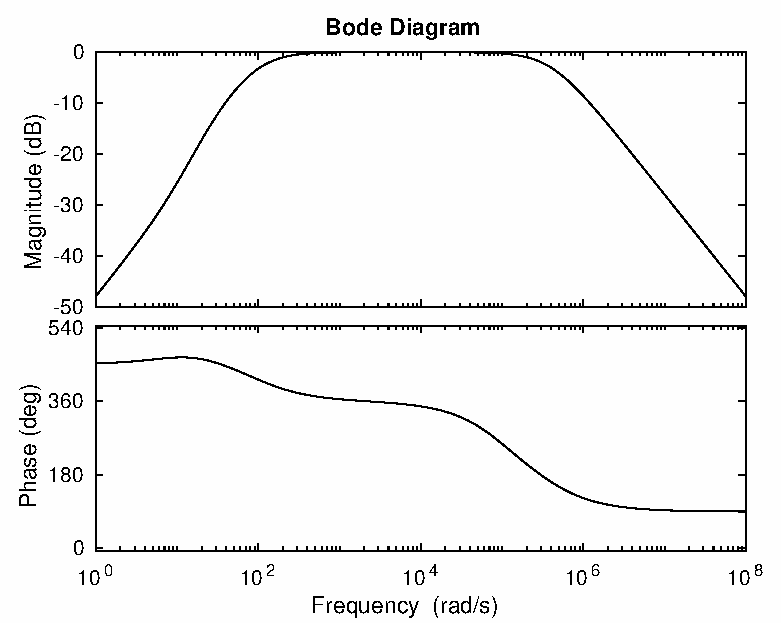
\includegraphics[width=0.45\linewidth]{p1_bode.eps}
	}
	\subfigure[Nyquist plot]{
		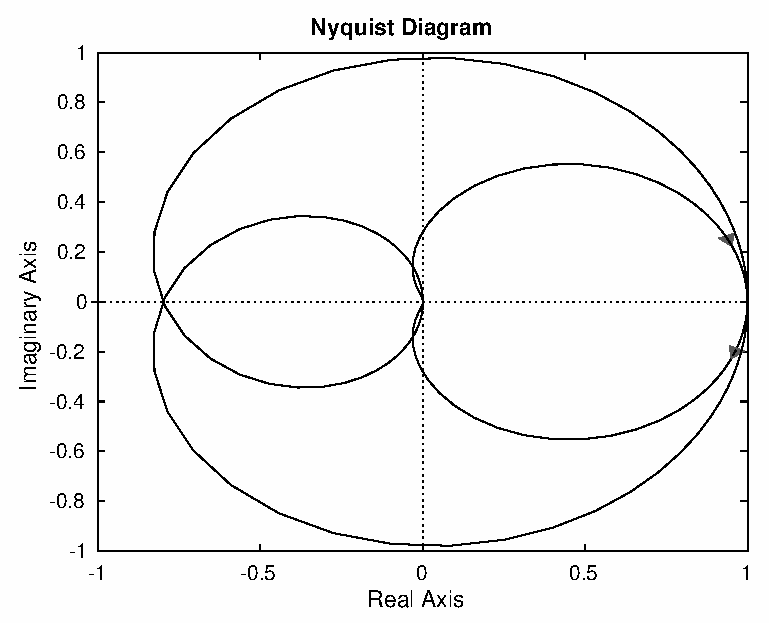
\includegraphics[width=0.45\linewidth]{p1_nyquist.eps}
	}
	\caption{Bode and Nyquist plot under $A_{mid}=1$.}
\end{figure}

\inputmintedindent{matlab}{p1.m}

\section{}
\begin{enumerate}
\item
Let $s=j\omega=j277$,
\begin{align*}
\frac{v_{L_2}(s)}{v_g(s)}
&=\frac{L_2s}{R+L_2s}\cdot\frac{(R+L_2s)\parallel(1/Cs)}{(R+L_2s)\parallel(1/Cs)+L_1s}\\
&=\frac{L_2s}{L_1L_2Cs^3+RL_1Cs^2+(L_1+L_2)s+R}\\
&=\frac{4\times10^{-3}s}{1.2\times10^{-8}s^3+6\times10^{-6}s^2+7\times10^{-3}s+2}\\
&\approx0.3584 + j0.3277\\
&\approx0.4856 \angle 0.7407
\end{align*}
$$v_{L_2}(t)=0.4856 \angle 0.7407 \cdot 10\sin(277t)=4.856\sin(277t+0.7407)$$

\begin{figure}[!htbp]
	\centering
	\subfigure[Bode plot]{
		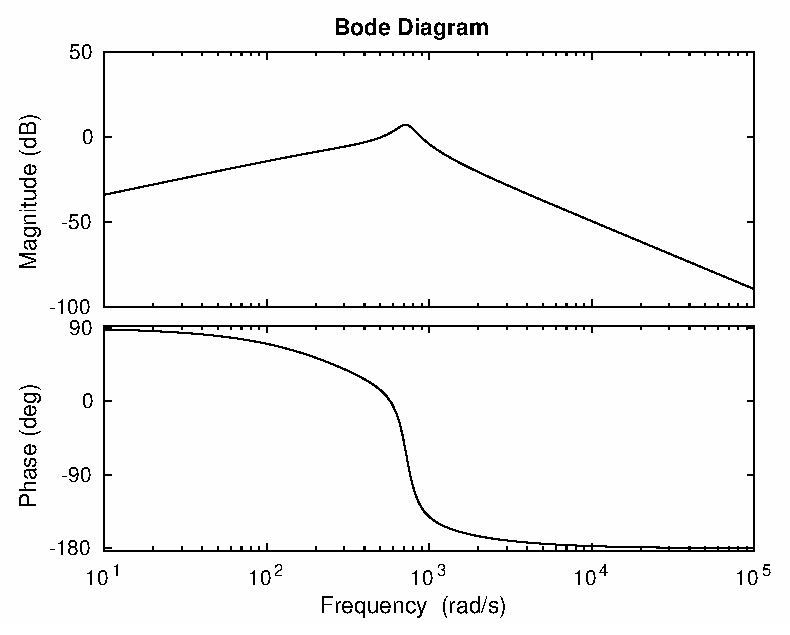
\includegraphics[width=0.45\linewidth]{p2_1_bode.eps}
	}
	\subfigure[Nyquist plot]{
		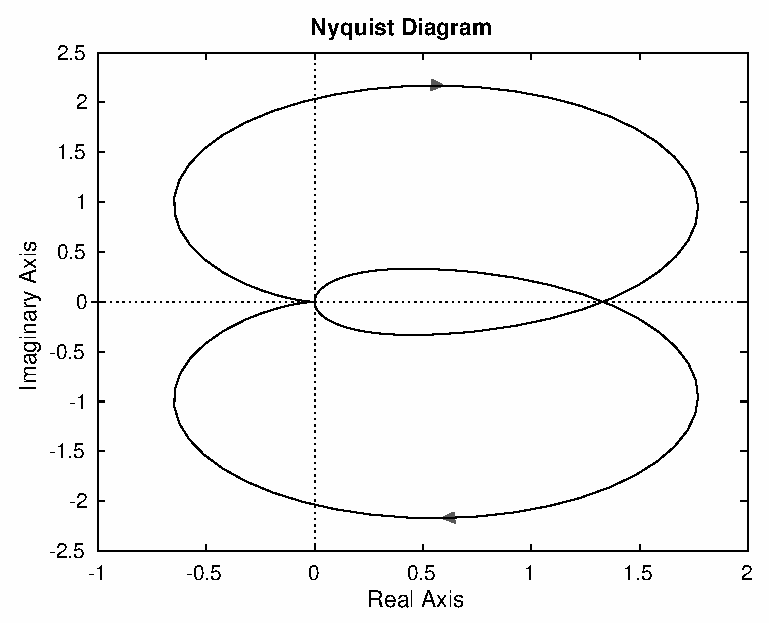
\includegraphics[width=0.45\linewidth]{p2_1_nyquist.eps}
	}
	\caption{Bode and Nyquist plot.}
\end{figure}

\inputmintedindent{matlab}{p2_1.m}

So the system is stable.

\newpage

\item
$$\left\{\begin{aligned}
-v_0+i_1R_1+\frac{1}{C}\int(i_1-i_L)dt&=0\\
\frac{1}{C}\int(i_L-i_1)dt+L\frac{di_L}{dt}+i_LR_2&=0
\end{aligned}\right.$$
$$-v_0+i_1R_1+L\frac{di_L}{dt}+i_LR_2=0$$
$$i_1=\frac{v_0}{R_1}-\frac{R_2}{R_1}i_L-\frac{L}{R_1}\frac{di_L}{dt}$$
$$\frac{i_L}{C}-\frac{v_0}{R_1C}+\frac{R_2}{R_1C}i_L+\frac{L}{R_1C}\frac{di_L}{dt}+L\frac{d^2i_L}{dt^2}+R_2\frac{di_L}{dt}=0$$
$$3\frac{d^2i_L}{dt^2}+11.5\frac{di_L}{dt}+15i_L=10v_0$$
$$3v_{R_2}s^2+11.5v_{R_2}s+15v_{R_2}=10v_0$$
$$\frac{v_{R_2}(s)}{v_0(s)}=\frac{10}{3s^2+11.5s+15}$$
$$v_{R_2}(s)=\frac{5\pi/s^2}{3s^2+11.5s+15}$$
$$v_{R_2}(t)=\frac{\pi t}{3}-\frac{23\pi}{90}+\frac{23\pi}{90}\exp\left(-\frac{23t}{12}\right)\left[\cos\left(\frac{\sqrt{191}t}{12}\right)+\frac{169\sqrt{191}}{4393}\sin\left(\frac{\sqrt{191}t}{12}\right)\right]$$

\begin{figure}[!htbp]
	\centering
	\subfigure[Bode plot]{
		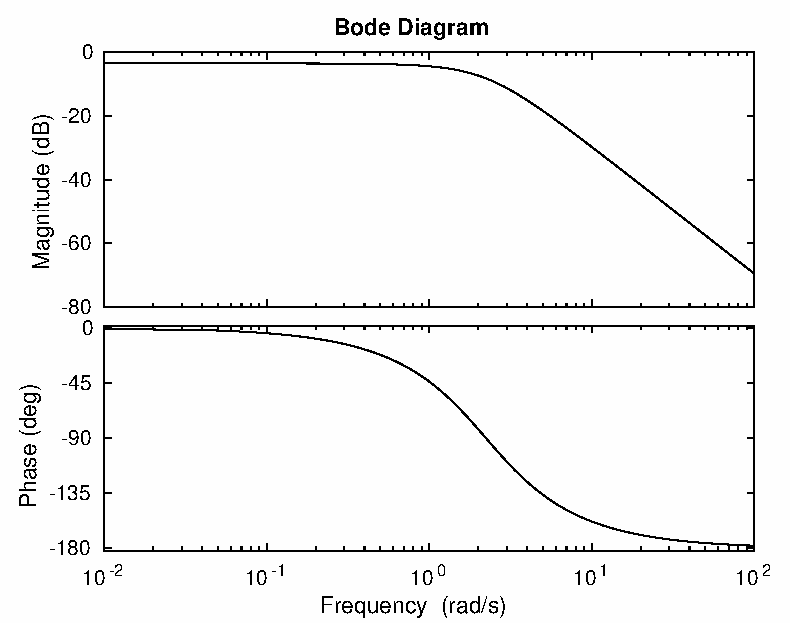
\includegraphics[width=0.45\linewidth]{p2_2_bode.eps}
	}
	\subfigure[Nyquist plot]{
		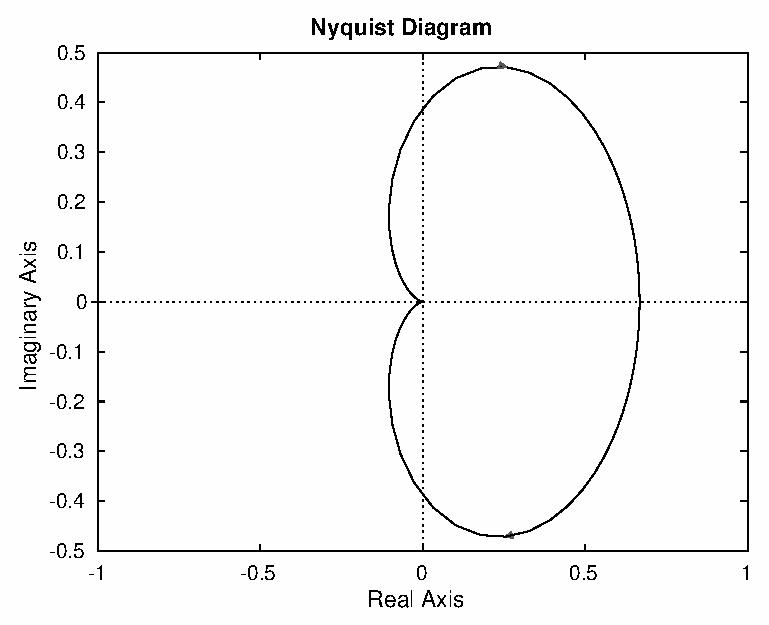
\includegraphics[width=0.45\linewidth]{p2_2_nyquist.eps}
	}
	\caption{Bode and Nyquist plot.}
\end{figure}

\inputmintedindent{matlab}{p2_2.m}

So the system is stable.

\end{enumerate}

\section{}
Let $s=j\omega$,
$$\frac{V_i}{R}=-\frac{V_1}{R\parallel(1/C_1s)}=-V_1\frac{R+1/C_1s}{R/C_1s}$$
$$\frac{V_1}{V_i}=-\frac{1/C_1s}{R+1/C_1s}=-\frac{1}{RC_1s+1}$$
$$\frac{V_2}{V_1}=-\frac{R}{R+1/C_2s}=-\frac{RC_2s}{RC_2s+1}$$
$$\frac{V_o}{V_2}=-\frac{R_f}{R_1}$$
$$\frac{V_o}{V_i}=\frac{V_1}{V_i}\cdot\frac{V_2}{V_1}\cdot\frac{V_o}{V_2}=-\frac{RR_fC_2s}{R_1(RC_1s+1)(RC_2s+1)}=-\frac{470s}{(47s+1)(0.2s+1)}$$

The poles are $\omega_{p_1}=-\dfrac{1}{47}\unit{rad/s}$ and $\omega_{p_2}=-5\unit{rad/s}$. The zeros are $\omega_{z_1}=0$.

\begin{figure}[!htbp]
	\centering
	\subfigure[Bode plot]{
		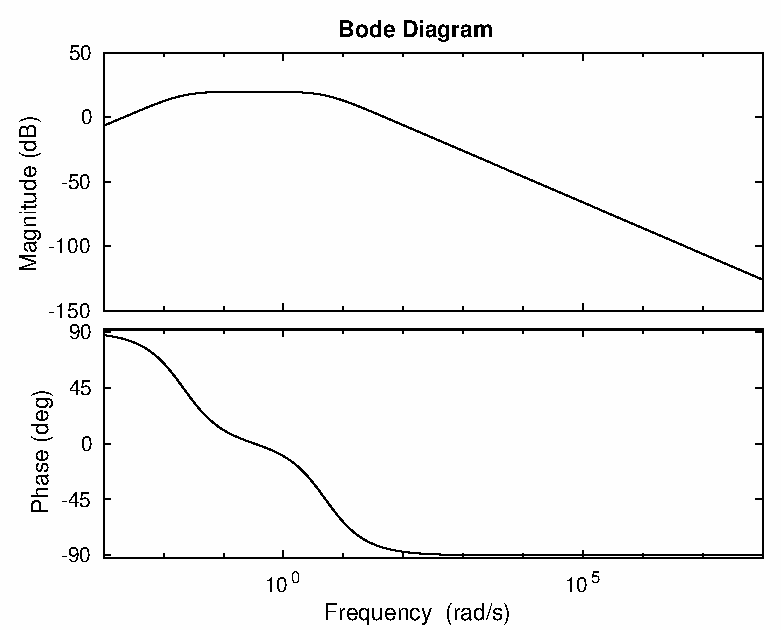
\includegraphics[width=0.45\linewidth]{p3_bode.eps}
	}
	\subfigure[Nyquist plot]{
		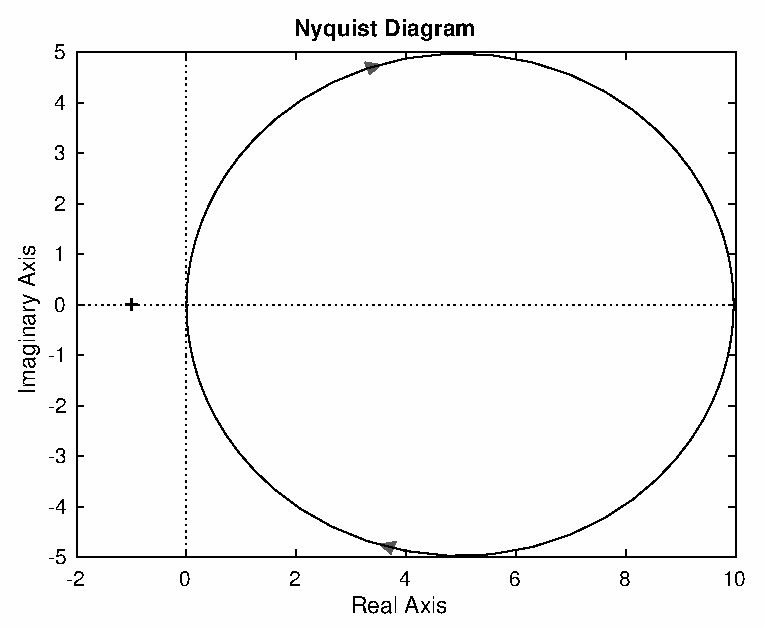
\includegraphics[width=0.45\linewidth]{p3_nyquist.eps}
	}
	\caption{Bode and Nyquist plot.}
\end{figure}

\inputmintedindent{matlab}{p3.m}

When $v_i=100\cos(600t)$, $$V_o=-\frac{470s}{(47s+1)(0.2s+1)}\cdot100\cos(600t)\approx\frac{1}{12}\angle\frac{\pi}{2}\cdot100\cos(600t)=\frac{25}{3}\sin(600t)$$

From the simulation, we found $v_o\approx11.96982\sin(600t)$.

The results are similar.

The SPICE code is \\

\inputmintedindent{v}{p3.cir}

The result is \\

\inputmintedindent{v}{p3.result2}
\end{document}

